% !TEX root = ../Thesis.tex
% !TEX spellcheck = en-US

\chapter{GNS3}
\label{ch:gns3}

GNS3, whose original title was ``Graphical Network Simulator-3,'' is a software project, comprising several distinct components and, despite the ``simulator'' in its name, \emph{as a whole}, it falls under the category that, in this thesis, is called \emph{emulator}. % TODO try to (either with a source, or speculating) relate the name with ns-3
% TODO also: cite the source for the name
By ``as a whole,'' it is meant that, as shall be seen later, although some of its components, like the Dynamips program, are emulators in a very strict sense---i.e. its purpose is to run real machine code on a different hardware architecture (than its native one)---, it differentiates itself, on a high-level perspective, from a simulator which is a program designed to execute a mathematical model, processing modeled events as internal data-structures with a collection of preset algorithms that somehow mimic (a part of) the reality.

It's important to notice that a necessary step towards the goal of this this thesis is to systematize a technical description of the architecture and functional underpinnings of the GNS3 system, how is it executed, how does it interact with the hardware and software it is running in, how much resources does it take to work with GNS3 according to the \emph{mode} it is running in, etc., as that is an aspect that is yet to be further explored for, at least, the following reasons:  % TODO improve the writing how is etc written in Engilsh?
for one, the consulted academic material (i.e. research papers, mostly) is very brief and omissive in regards to the design, architecture and implementation of GNS3, and so is the official website and documentation. Besides that, many interesting details are in the ``paraofficial'' videos available via YouTube, but certified as official, by David Bombal\footnote{\url{https://www.youtube.com/channel/UCP7WmQ_U4GB3K51Od9QvM0w}}, namely a comprehensive overview of the architecture (compared with the functionality) of GNS3 by its creator, Jeremy Grossmann, and essentially are not anywhere else, at least from authoritative sources. % TODO same as the previous "sentence". Cite the videos (how and which ones?)

% TODO add a figure (a screen shot) showing the "official" submitter of GNS3 videos (and maybe the channel and/or links from the gns3 official website)

% end of intro

\section{GNS3's purpose and \emph{raison d'être}}
\label{sec:gns3why}

The GNS3 project was co-created by Jeremy Grossmann at the University, the EPITECH, as part of the \emph{EPITECH Innovative Project (EIP)}\footnote{\url{https://eip.epitech.eu/2013/gns3/en/index.html}, accessed on December 2019}.
There is also a blog\footnote{\url{http://gns3.blogspot.com/2007/}, accessed on December 2019}, whose first posts date of 2007, that announces the first ``beta'' releases of the software and gives the details about the inception of GNS3, and also shows lists the original developers of the project. In particular, it is clearly stated the dependency on Dynamips, a program that will be explored later, and that currently is under the process of being deprecated.

It may be speculated that GNS3's first ``appeal'' was supplying students of Cisco certifications with a self-study tool more powerful that anything before, one that allows for the creation of arbitrary network topologies and practice their skills with the same software stack that is used in real Cisco devices and the hosts connected to them---from the operating system, up until application--level network utilities---, without having to use the expensive official solutions for that purpose, or depending on a real, physical networking laboratory, or having to fall back on the limited graphical simulators like Cisco's Packet Tracer.
However, despite having kept a strong relation with training for Cisco CCNA and related certifications, the magnitude of the project, part of which comes from an inherent extensibility, has made it suitable for a myriad of use-cases.

In the industry, GNS3 naturally can come handy as a tool to prototype and test a topology for a real organization network, in the context of the practice of a network professional. But also, in the age of the DevOps philosophy---a set of practices and methodologies/philosophies for faster delivery of applications and services---, of which \emph{infrastructure as code} is one of the culprits~\cite{awswhatisdevops}, it can be of value for software engineers to test distributed applications that depend on certain network behaviors. Use cases related to cybersecurity are abundant (one kind of node that is available to add to GNS3 \emph{topologies} are firewalls), as well as for usage in the context of \gls{SDN}.
But also potential applications that are still relatively unexplored, such is the case of its usage in teaching and learning, particularly in the undergraduate and graduate university levels (and schools), the focus of of this work.

At the moment of the writing of this thesis, version 2.2 has recently came out\footnote{\url{https://github.com/GNS3/gns3-gui/releases/tag/v2.2.0}}.
This version brings a lot of improvements and new features, like the new web UI or ``physical'' link state detection for QEMU nodes~\cite{releasenotesgns3v22}, and at the same time some of the ways GNS3 has been typically used are changing.
Such is the case of the discouragement of the usage of Dynamips and VPCS (in detriment of virtualized versions of IOS or others, or Docker containers for ``emulating'' hosts, respectively)~\cite{ytdynamipsvpcs}.


\section{Building blocks. The programs ``inside'' GNS3}
\label{sec:gns3buildingblocks}

In an very simplified way of summarizing it, GNS3 is a conjunction of UI tools (the official GUI, the new web UI, or any custom program that ``speaks'' the documented public \acrshort{REST} API), a powerful distributed orchestrator (the \emph{controller} in the server), and a set of integrations (the so-called ``compute nodes'') with virtualization, containarization, and emulation tools from ``the outside'', i.e. that do not belong to the GNS3 project, like KVM, Docker, or QEMU, to provide a way to describe a topology of interconnected computing and routing nodes---that is, a computer network---, including firewalls and NAT devices, control their behavior and launch administrative tools (like \texttt{telnet} sessions). % TODO cite documentation of the REST API. Make sure we elaborate on "computes". How is so-called written - is an hyphen used?

What follows is a description of what are those elements and what they do work internally.
How they integrate with GNS3 or vice-versa, and also how they interact with each other, is described in~\ref{sec:gns3architecture}.

\begin{figure}
  \centering
  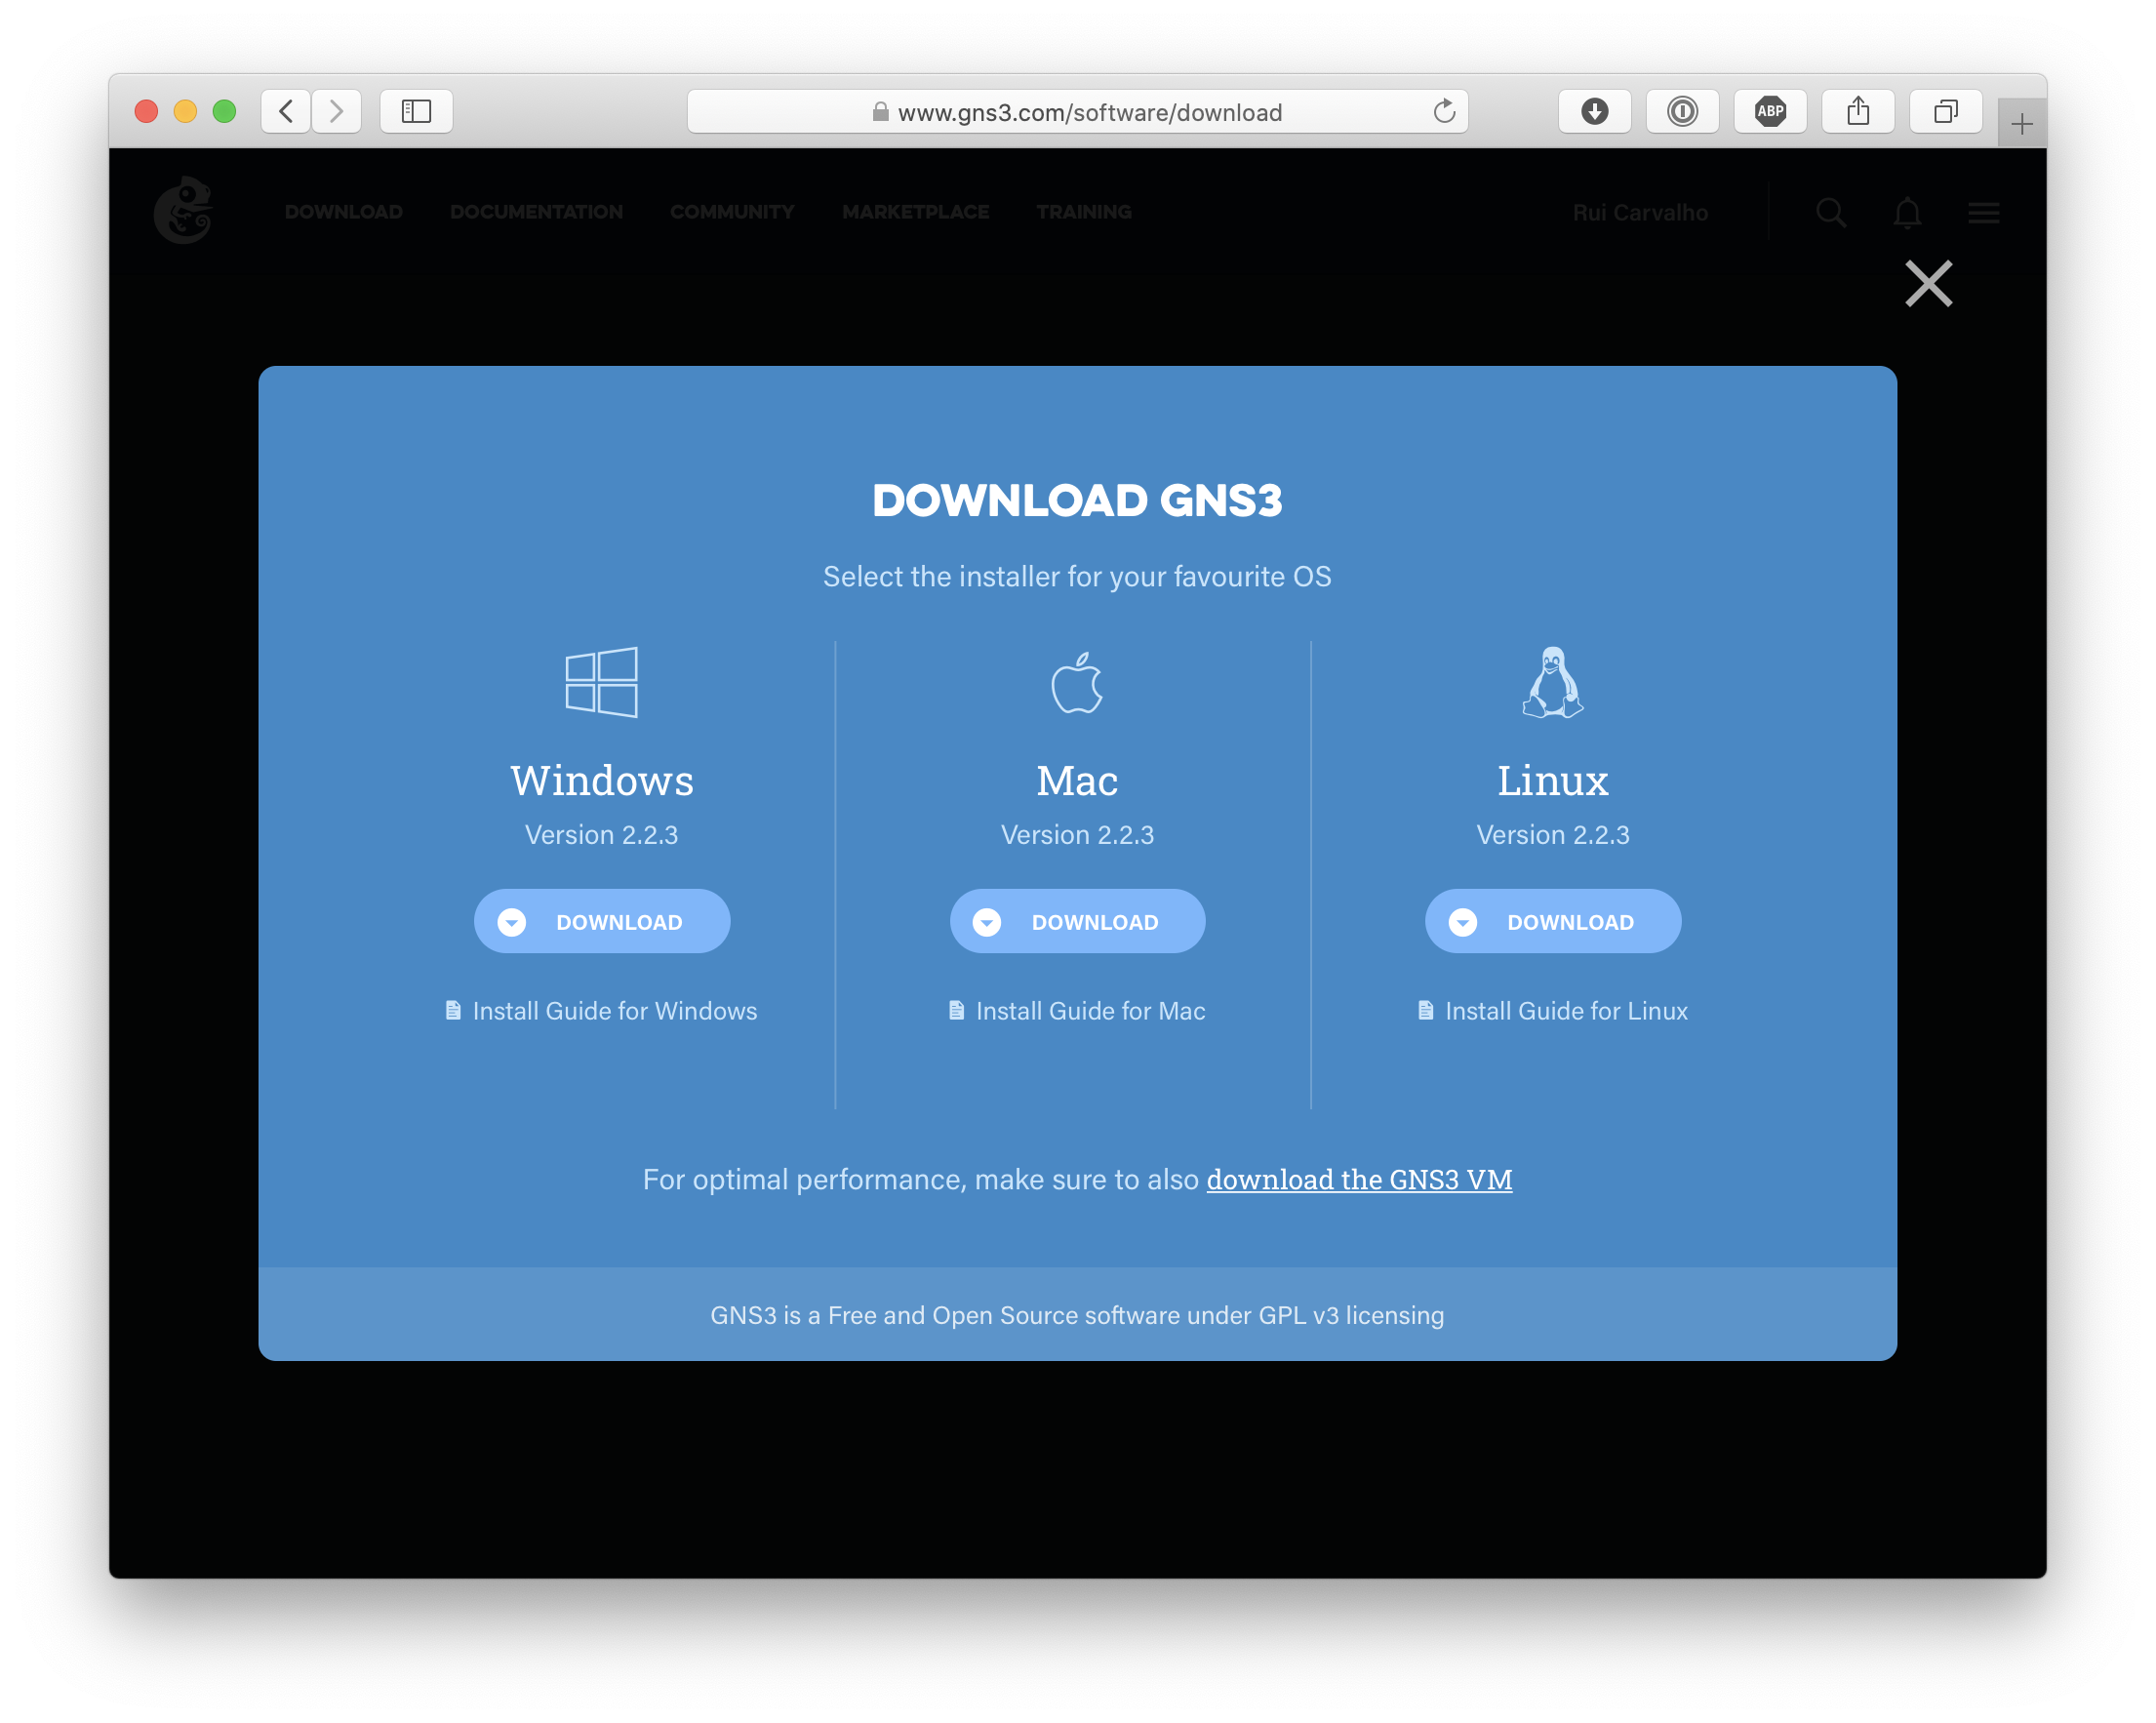
\includegraphics[width=0.8\textwidth]{download-gns3}
  \caption{The download screen on the official GNS3 website}
  \label{fig:download-gns3}
\end{figure}

When GNS3 is installed downloading one of its desktop distributions---available for Windows, macOS, and GNU/Linux, like the screen shot~\ref{fig:download-gns3} shows---, a user is installing multiple ``programs'' (or applications, whichever is the preferred denomination), implemented in disjunct \emph{codebases}, and, given that they are \emph{free and open source} projects~\cite{gplv3}, hosted in GitHub, those \emph{codebases} are easily accessible---and developers can enhance features and provide bugfixes. Those are the essential building blocks of GNS3 and table~\ref{tab:gns3components} can serve a summary of what those pieces are.
It's worth noting that they are all under the GNS3 organization in GitHub\footnote{\url{https://github.com/gns3}}.

\begin{table}
  \centering
  \small
  \begin{tabulary}{0.8\textwidth}{lLL}
    \toprule
      \textbf{Part}  & \textbf{Role}                                                       & \textbf{Source code repository}\\
    \midrule
      GNS3 GUI       & A desktop application that runs on a graphical OS                   & \scriptsize\url{https://github.com/GNS3/gns3-gui}\\
      Dynamips       & A MIPS emulator, used by the \emph{backend} to run (old) IOS images & \scriptsize\url{https://github.com/GNS3/dynamips}\\
    \bottomrule
  \end{tabulary}
  \caption{%
    Intrinsic parts of GNS3, constituting separate and independent codebases
  }
  \label{tab:gns3components}
\end{table}


\subsection{GNS3 GUI}
\label{subsec:gns3gui}

Interaction between the end-user and GNS3 is usually---though, as will be clear, not necessarily---done in a graphical environment.
A GNS3 project, called a \emph{topology}, is constantly opened on one single window (per running instance of the application) and is graphically represented in the main section of the window.

Even though the GUI is not the authoritative source of truth for a topology (cf.~\ref{sec:gns3architecture}), it can be used as interface to all of GNS3's functionality: edit the topology itself (adding or removing nodes, changing links), performing actions on the nodes (like starting or stopping a host or router), or using helpers to launch consoles automatically connected via \texttt{telnet} or SSH.
In the section dedicated to the usage of GNS3~\ref{sec:gns3inaction}, it will be shown how this is done from a user's perspective.
Many GUI clients, on different hosts (e.g. laptops), can be editing the same topology at the same time. % TODO try to capture screenshots of this happening (use VMs)

\begin{figure}
  \centering
  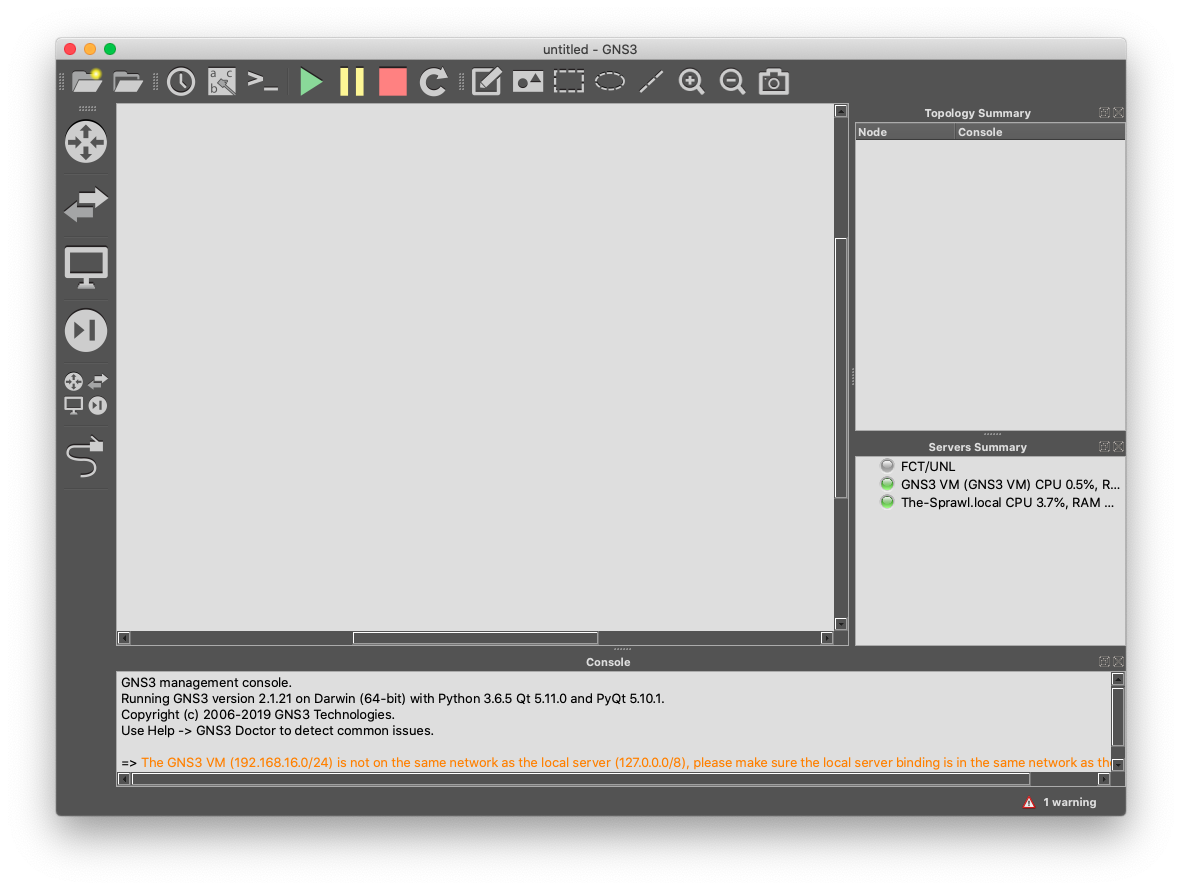
\includegraphics[width=0.8\textwidth]{gns3-empty-topology}
  \caption{An empty GNS3 topology shown in the GUI}
  \label{fig:gns3-empty-topology}
\end{figure}

\subsection{Dynamips}
\label{subsec:gns3dynamips}

The Dynamips emulator is a standalone program, written in C, that, usually, comes distributed together with the whole GNS3 package.
It is an emulator for a MIPS processor and was the original--single way to run the software of the Cisco nodes of the topologies created with GNS3.


\subsection{GNS3 server}
\label{subsec:gns3server}


\subsection{GNS3 VM}
\label{subsec:gns3vm}

% end of section gns3buildingblocks

\section{General architecture}
\label{sec:gns3architecture}

\begin{figure}
  \centering
  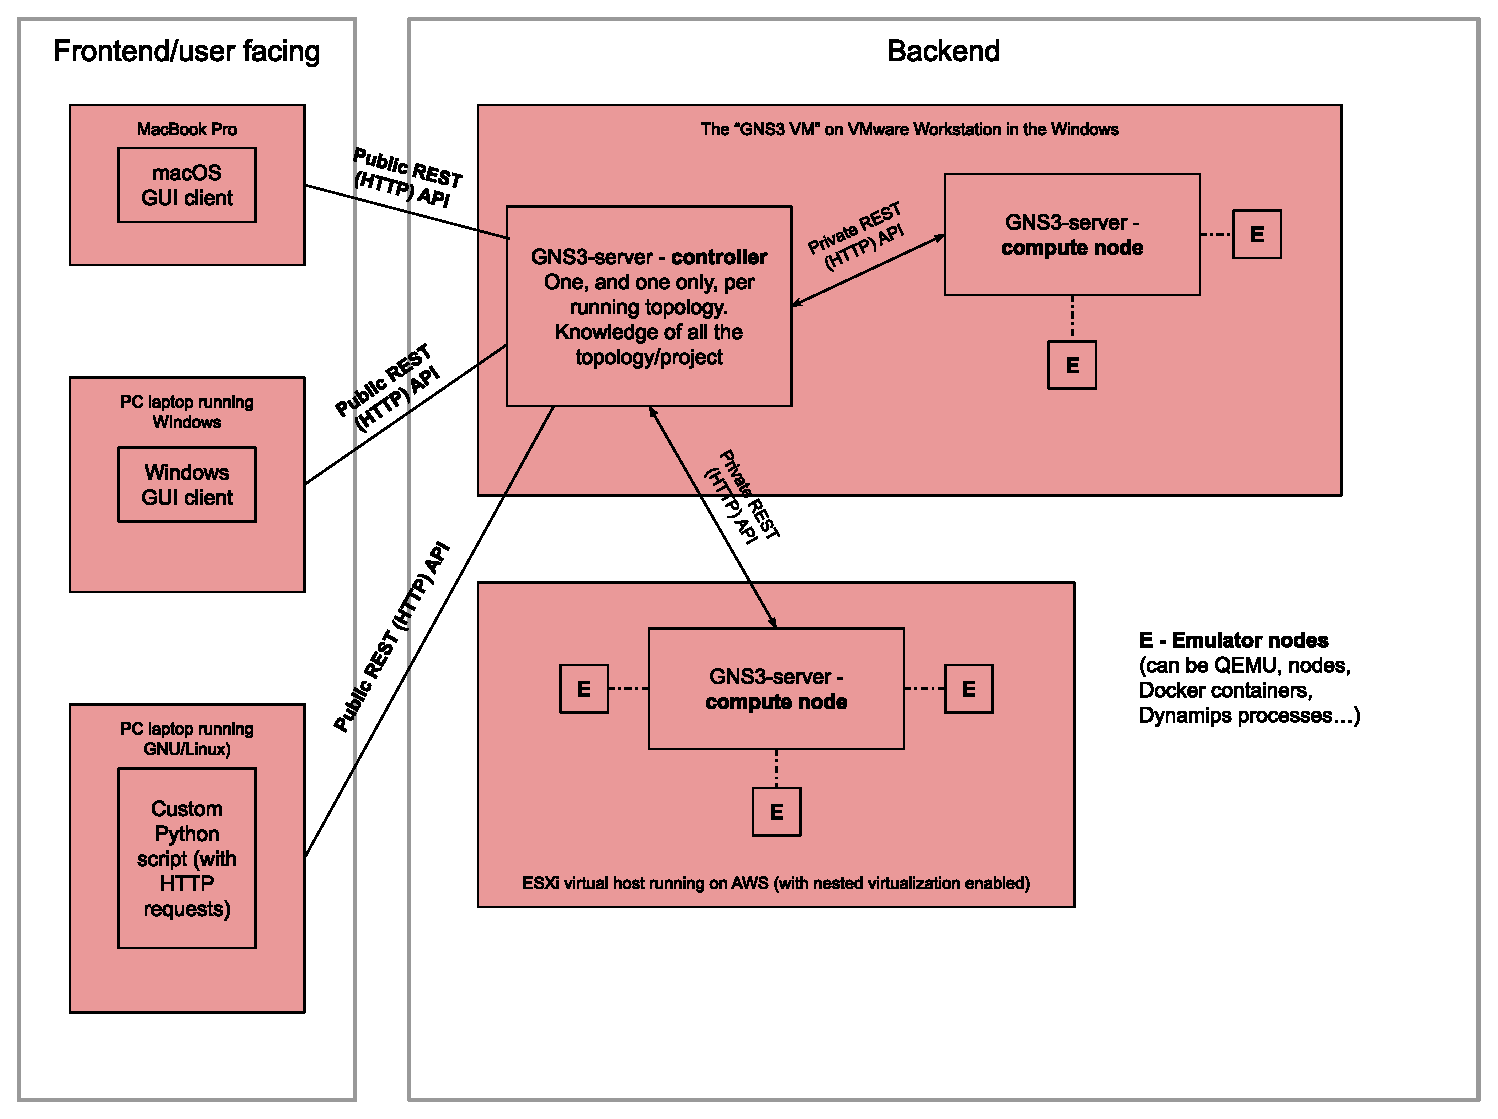
\includegraphics[width=1\textwidth]{gns3-running-arch}
  \caption{The GNS3 architecture}
  \label{fig:gns3-running-arch}
\end{figure}

In this section, an attempt is made to describe the different parts of GNS3 is to see what role they play in an execution of a topology (i.e. a project) and how they communicate with each other.
The diagram in figure~\ref{fig:gns3-running-arch} is based upon~\cite{ytgns3arch22}.
A central idea is the potentially distributed nature of the components, allowing for a complex topology with many nodes to be run across many hosts, dividing the computing power load across more than one host.
The precautions that must be taken to ensure a performance, and some caveats, will be explained in~\ref{sec:gns3inaction}. % TODO precautions taken?

The GNS3 server program, described in subsection~\ref{subsec:gns3server}, has two roles in a GNS3 session. % TODO define what's a "GNS3 session"
Those are: ``computes'' and the controller.
A GNS3 session only has one controller.
Any desktop installation of GNS3 comes with the server installed, able to run as the controller.
The GNS3 GUI will connect to the controller and allow for the user to ``open'' a topology on it.
The communication, as said, between any client (the GUI or any script) and the controller happens through HTTP requests following a REST approach. % TODO link acronyms et al to gls
The controller has knowledge of all the hosts running nodes of the topology.
Those nodes are run using ``computes'', which are processes of the GNS3 server whose responsibility is to expose a private REST API---\emph{not the same} as the one that the controller exposes and only to be used internally--- to receive commands from the decision point (the controller) and locally interact with QEMU processes, Docker containers, Dynamips processes, or other emulation, container, or virtualization solution over which a node of the topology (an IOS Cisco router, a host, or a NAT node) is executed.

Therefore, on the diagram depicted in figure~\ref{fig:gns3-running-arch}, we see a topology running on distributed machines---these could be exclusively interconnected virtual machines on the same physical computer, without any loss of generality. % TODO put the background of the word of the same color that it has on the diagram
What matters is that they are running in hosts able to communicate with each other via IP and where GNS3 server is supported.
Each magenta rectangle is a separate host. % TODO check the color name
On the backend there are two hosts.
One of the hosts is the ``GNS3 VM'', running over VMware Workstation for Windows, and is ``playing'' both roles of the GNS3 server at the same time: it is the (single) controller for the running topology, which means that it loads the file describing the topology and has the receives the client's input, while knowing on which host should each topology node by run.
Then, it has a compute running alongside, to run two topology nodes.
These can be, for example, Cisco IOSv routers. % TODO how to spell IOSv. Somewhere we need to talk about this
On another host, which is a ESXi virtual machine (running on some infrastructure), \emph{with nested virtualization enabled}, the GNS3 server is also running, but there is no controller---all it does is ``blindly'' (at specific requests from the controller via the private REST API) execute, in the compute nodes, the necessary local interactions with the emulators. % TODO ESXi cite/link something
In the picture, there are three nodes running, which can be, for example, a Dynamips emulator for a <supported Dynamips Cisco router> and two hosts running on Docker. % TODO replce with a real model

% end of section gns3architecture

\section{GNS3 in action}
\label{sec:gns3inaction}

% end of section gns3inaction

\section{Performance and resources considerations}
\label{sec:gns3performance}

% end of section gns3performance

% end of chapter
